\chapter{Results}

% What I want to say
%     - we see that there are differences between tokenizers on the metrics
%         - tokenizer method influences vocabulary allocation
%              - algorithm, and even implementation
%              - definitely compare my unigram / huggingface unigram to show the difference
%         - alpha factor influences vocabulary allocation
%         - data size influences vocabulary allocation but converges
%         - tokenizer influences vocabulary overlap but 
%         - data size influences vocabulary overlap but also converges
%     - 
% now with the knowledge of differences, lets compare the Limi unigram, Limi bpe and tokmix
% we see that the metrics correlate with the downstream tasks. Although there are task-specific differences
% - therefore cpt, ar, jsd are good metrics for comparing tokenizers

% - we can see that all balancing methods do influence the quality of the tokenizers on languages
% - we observe that all balancing methods produce similar improvements on lowresource
% - we check this by comparing the balancing methods on downstream and we do not see any significant differences between them. We do see improvements over the strong baseline in some cases.
% - therefore we can conclude that balancing does influence NER and POS tagging although with the comparison to alpha0.3, the improvements are very small


\section{The effects that influence the tokenizers quality}


\subsection{Vocabulary allocation of tokenizers}
\subsubsection{Tokenizer methods and vocabulary allocation}

% \subsubsection{Data size and vocabulary overlap}
% this is included in the data_size_influence table

\section{The influence of vocabulary allocation and overlap on the language representation quality}

Firstly, we see that the default settings of the Huggingface tokenizers produce very different alphabet sizes and in turn affect the UNK rate. As we will see later, this does not affect the metrics significantly.


\begin{figure}[H]
    \centering
    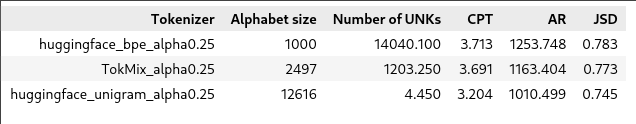
\includegraphics[width=\textwidth]{img/temp/20l_metrics.png}
    \caption{In the first batch of experiments, we compare the Huggingface tokenizers and our TokMix method based on merging Unigram tokenizers. Huggingface Unigram has significantly lower vocabulary allocation scores (CPT and AR) than BPE and TokMix. This means that Unigram uses shorter tokens and the capacity of the vocabulary is used less uniformly. Moreover, the vocabulary has more overlap (lower JSD) between the languages for Unigram. This might be related to the low allocation as it is more likely that shorter tokens are shared between languages. The scores are macro averages over all languages.}
    \label{fig:20l_metrics}
\end{figure}


\begin{figure}[H]
    \centering
    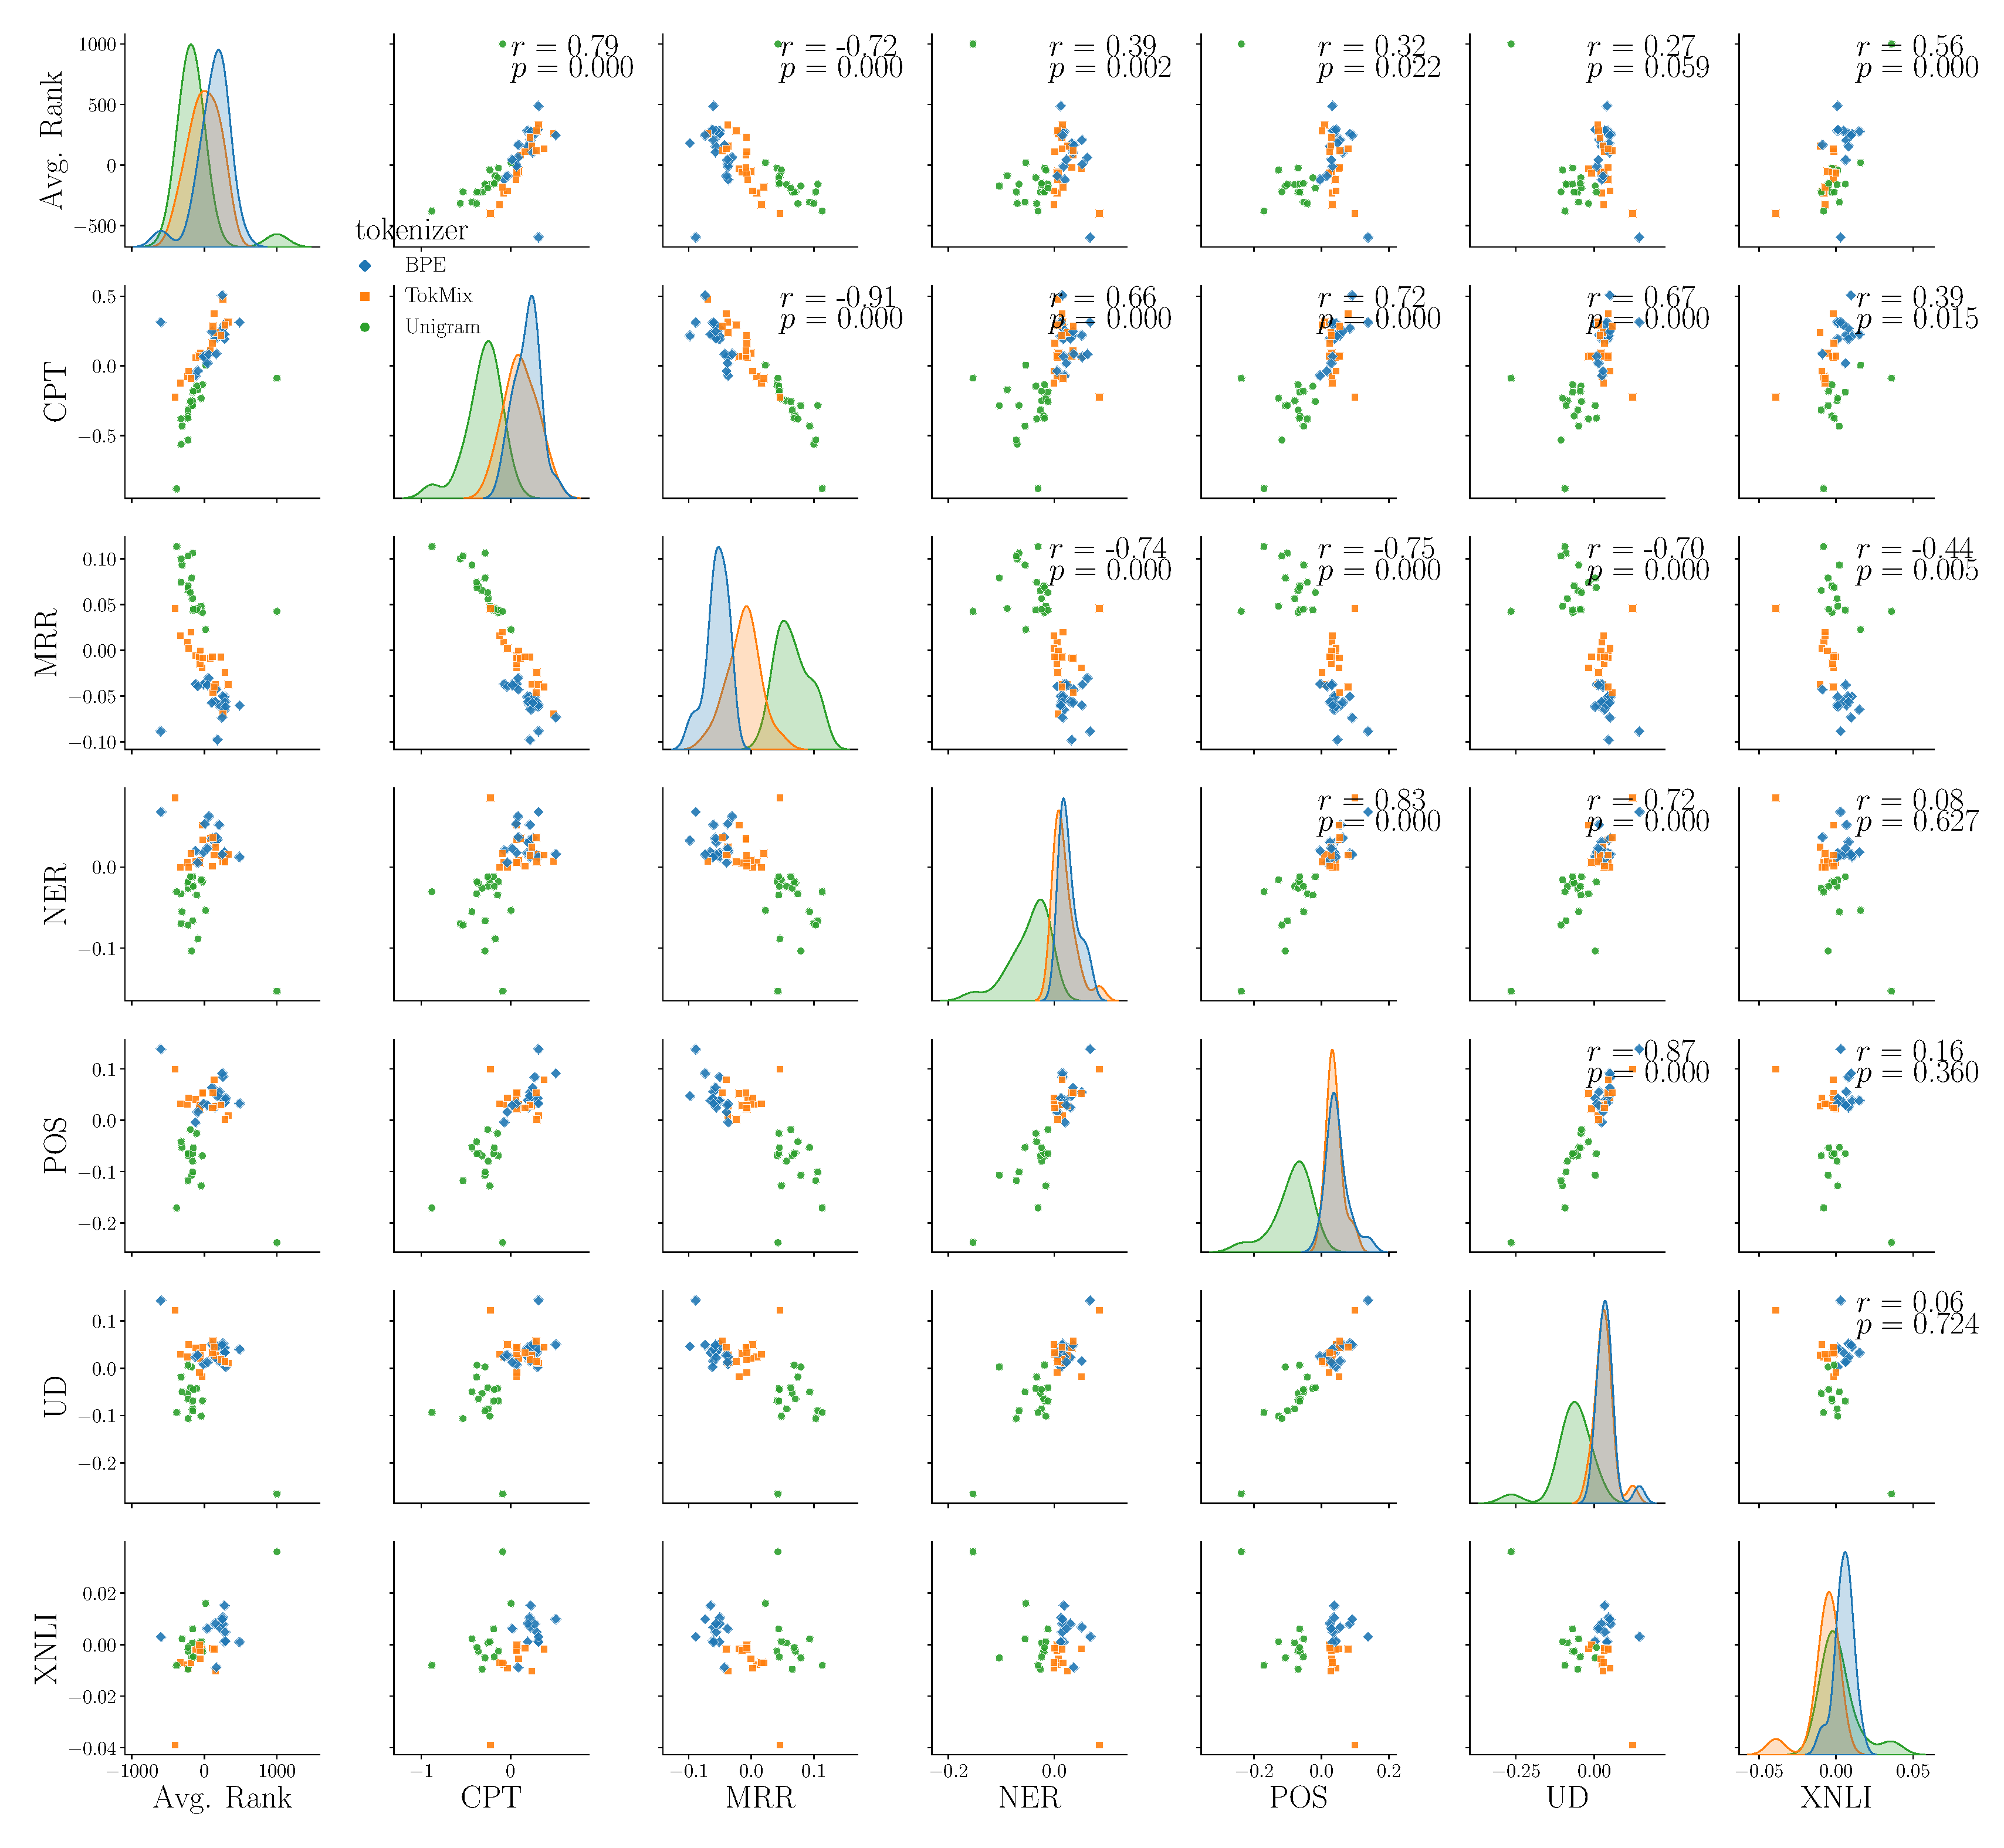
\includegraphics[width=\textwidth]{paper/figures/pair_analysis_20L.pdf}
    \caption{We compare the tokenizer metrics against the downstream task results. For each tokenizer we pretrain a masked language model and finetune it on each of the available languages. We observe high spearman correlation between CPT and the word-level tasks (NER, POS, UD) and high correlation between AR and the sentence-level task XNLI. This suggests that our vocabulary allocation metrics are good indicators of the tokenizers quality and higher vocabulary allocation leads to better downstream performance. Each data point corresponds to an average result over three seeds of finetuning and evaluating on one of the languages. The results for each language are centered around the mean to account for the differences between languages.}
    \label{fig:pair_analysis_20L}
\end{figure}

\begin{figure}[H]
    \centering
    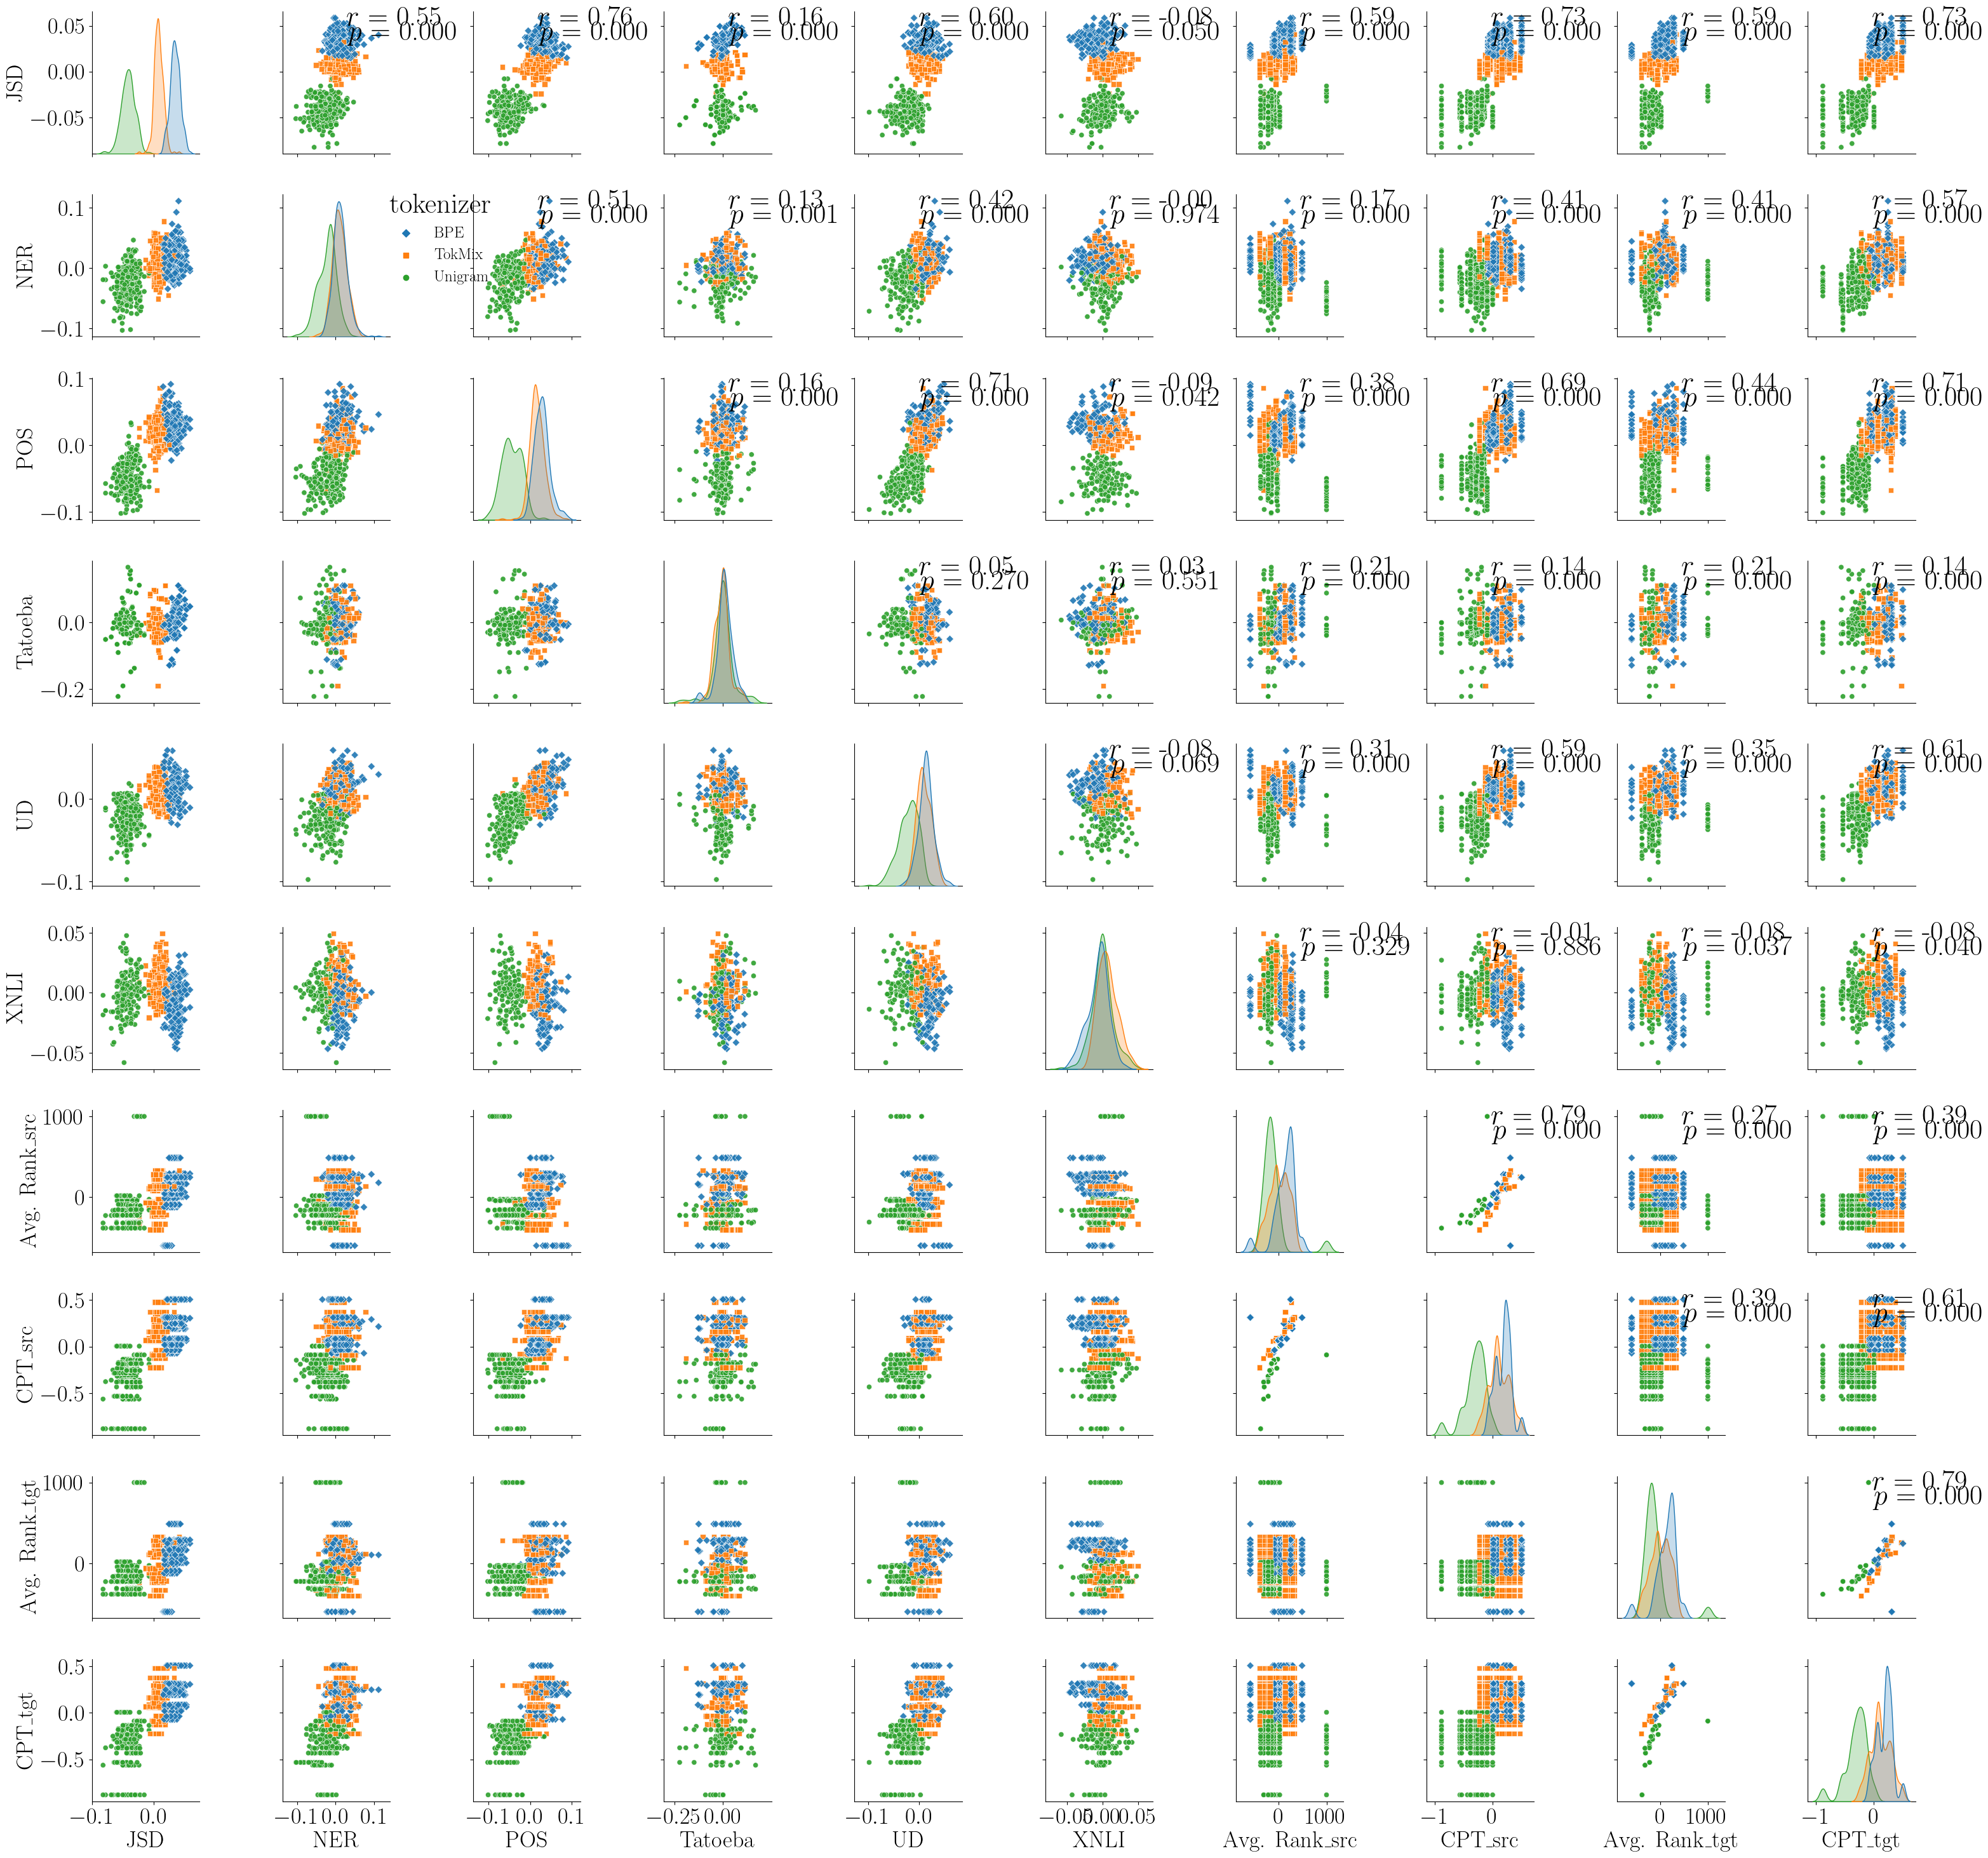
\includegraphics[width=\textwidth]{img/temp/X_pair_analysis_20L.png}
    \caption{We compare the tokenizer metrics against the cross-lingual performance of the models. For each tokenizer we pretrain a masked language model and finetune it on each of the available languages. Then we evaluate the models on all languages it has \textbf{not} been finetuned on, assessing the cross-lingual properties of the model. Here we observe high correlation between JSD and the word-level tasks, especially the POS and UD. This suggests that less overlap (higher divergence) between the vocabularies of the languages leads to better cross-lingual performance.
    \xxx{remove the ar and cpt metrics?}}
    \label{fig:X_pair_analysis_20L}
\end{figure}

\begin{table}
\centering

\begin{tabular}{lccc}
\toprule
 & \multicolumn{2}{c}{\bf{V. Allocation}} & \bf{MLM} \\
 & (AR) &  (CPT)  &  (MRR) \\
\midrule
CPT    &    \bf{0.790} &     - &  - \\
MRR    &  \bf{-0.723} &  \bf{-0.913} &  - \\
NER    &   \bf{0.394} &   \bf{0.657} &  \bf{-0.745} \\
POS    &     0.320 &   \bf{0.724} &  \bf{-0.754} \\
Dep l. &     0.266 &   \bf{0.675} &  \bf{-0.695} \\
NLI   &    \bf{0.56} &    0.388 &  \bf{-0.437} \\ 
\bottomrule
\end{tabular}
\caption{Spearman correlations between centered in-language task results and tokenizer measures. Statistically significant correlations ($p<0.01$) are bolded. Computed for 20 languages.}
\label{tab:corr_in_lang_20l}
\end{table}

\begin{figure}[H]
    \centering
    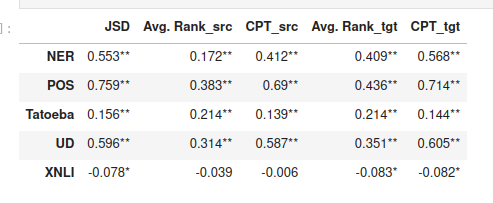
\includegraphics[width=\textwidth]{img/temp/corr_x_lang_20l.png}
    \caption{Correlations between task cross-lingual transfer results and tokenization measures."Stars denote statistical significance: (* coresponeds to $p<0.05$ and ** to $p<0.01$).\xxx{remove the ar and cpt metrics? Merge with the previous correlation table?}}
    \label{fig:corr_x_lang_20l}
\end{figure}

% ---------


\subsubsection{Data balance and vocabulary allocation}

\begin{figure}[H]
    \centering
    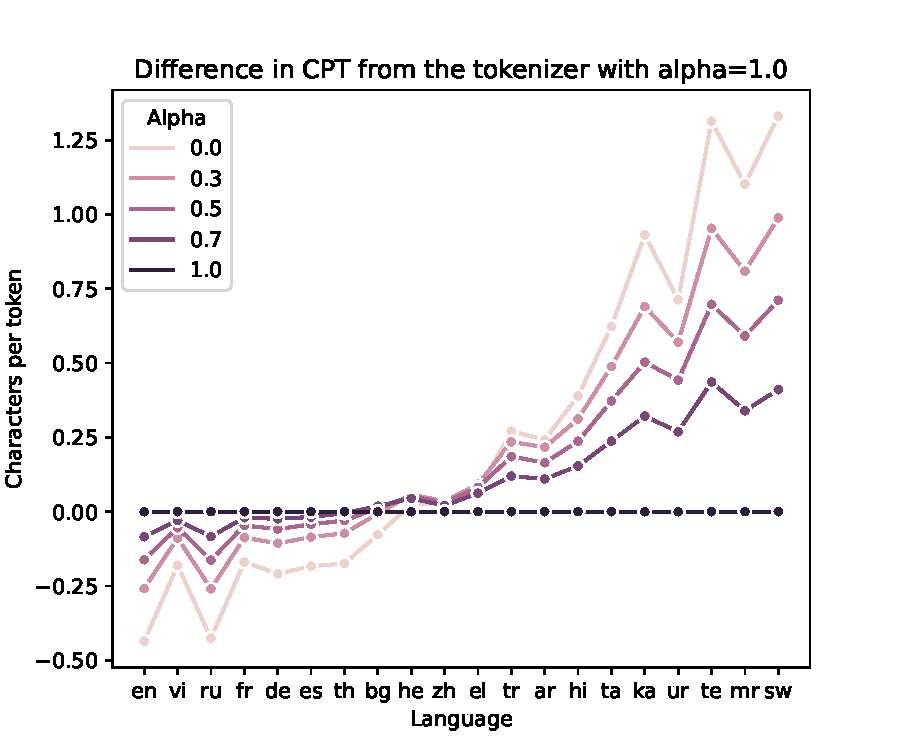
\includegraphics[width=\textwidth]{img/results/cpt_vs_alpha.pdf}
    \caption{fefefef.}
    \label{fig:num_lines_per_language_vs_cpt}
\end{figure}

\subsubsection{Data size}

\begin{table}
\centering
\caption{We measure how much data is generally needed for the tokenizer training. We train handful of Sentencepiece Unigram tokenizers on different amounts of balanced multilingual data. We observe that after 100k-1M lines per language, the tokenizers converge to similar vocabulary allocation and overlap scores. The significance of this experiment is that we find out experimentally how much data is needed for the tokenizer training and we can use this information to make sure that we provide enough data for each language for the further experiments.}
\label{tab:data_size_influence}
\begin{tabular}{rrrrrr}
\toprule
 Lines per language &  Alphabet size &  Number of UNKs &      CPT &          AR &      JSD \\
\midrule
               1000 &           3598 &          520.35 & 3.301636 &  958.414048 & 0.765687 \\
              10000 &           4725 &          117.75 & 3.597563 & 1089.112498 & 0.765236 \\
             100000 &           5041 &           65.55 & 3.695797 & 1192.201089 & 0.767133 \\
            1000000 &           5079 &           62.60 & 3.702038 & 1204.659073 & 0.767357 \\
            1500000 &           5176 &           55.90 & 3.705119 & 1210.664835 & 0.767348 \\
            2000000 &           5180 &           56.35 & 3.705109 & 1212.489940 & 0.767327 \\
\bottomrule
\end{tabular}
\end{table}


\subsubsection{Character coverage}

\begin{table}
\caption{We check the tradeoff of including a large alphabet size. We train Sentencepiece Unigram tokenizers with a different target character coverage and observe the resulting alphabet size, number of UNKs and tokenizer metrics. We observe that the alphabet size grows with the coverage and the number of UNKs decreases, as expected. We observe that at both extremes of the character coverage parameter, the vocabulary allocation decreases. The results indicate that the alphabet size between 1000 and 5000 provides a good tradeoff between the number of UNKs and the allocation metrics, while including all characters in the alphabet does not come with a significant decrease in the allocation metrics (-0.05 CPT).}
\label{tab:coverage_influence}
\begin{tabular}{lrrrrr}
\toprule
Coverage & Alphabet & \# UNKs & CPT & AR & JSD \\
\midrule
98.0\% & 539 & 17386.5 & 3.631 & 1115.3 & 0.749 \\
99.5\% & 1136 & 7786.9 & 3.702 & 1173.1 & 0.765 \\
99.95\% & 2678 & 910.6 & 3.705 & 1196.7 & 0.768 \\
99.995\% & 4813 & 83.0 & 3.695 & 1188.7 & 0.769 \\
99.9995\% & 8226 & 10.2 & 3.678 & 1164.2 & 0.769 \\
100.0\% & 13658 & 1.9 & 3.650 & 1124.1 & 0.768 \\
\bottomrule
\end{tabular}
\end{table}


\section{Comparison of balancing methods}
\subsection{Balancing methods and vocabulary allocation}

\begin{table}
\caption{In this summary table, we present all tokenizers used in this chapter. Along with the Huggingface tokenizers from table \ref{fig:20l_metrics} and Sentencepiece Unigram tokenizers from \ref{fig:data_balance_vs_allocation_per_lang}, we include the tokenizers obtained by replicating the papers \citet{chung_improving_2020,zheng_allocating_2021,liang_xlm-v_2023} in our setting. As we can see, the Huggingface Unigram tokenizer is a clear outlier in terms of all metrics even after taking account the higher alphabet size as explored in \ref{tab:coverage_influence}. Further we can see that the proposed balancing methods are improving over the baselines the authors used (\textit{unigram\_alpha0.5} and \textit{unigram\_alpha0.7}). On the other hand we see that using more balanced data for training the Sentencepiece Unigram (\textit{unigram\_alpha0.0}) does lead to similar overall performance as the replicated methods.
The rows are sorted by the CPT score. \xxx{As we can see that except for the Huggingface tokenizers, the alphabet sizes for all tokenizers stay in the stable range of 1000-5000. This corresponds to a comparable number number of UNKs in the holdout data.
}}
\label{tab:all_tokenizers_metrics}
\begin{tabular}{lrrrrr}
\toprule
Tokenizer & Alphabet & \# UNKs & CPT & AR & JSD \\
\midrule
huggingface\_bpe\_alpha0.25 & 1000 & 14040.1 & 3.713 & 1253.7 & 0.783 \\
unigram\_alpha0.0 & 2975 & 617.1 & 3.712 & 1212.9 & 0.767 \\
Chung\_20clusters & 4123 & 270.3 & 3.702 & 1098.7 & 0.766 \\
unigram\_alpha0.3 & 2666 & 923.5 & 3.702 & 1190.7 & 0.768 \\
TokMix\_alpha0.25 & 2497 & 1203.2 & 3.691 & 1163.4 & 0.773 \\
Chung\_16clusters & 3933 & 387.1 & 3.677 & 1102.2 & 0.767 \\
Liang\_20clusters & 3709 & 341.4 & 3.676 & 1103.2 & 0.765 \\
Zheng\_20langs & 4854 & 245.7 & 3.673 & 1094.5 & 0.765 \\
Liang\_16clusters & 3655 & 416.8 & 3.669 & 1106.2 & 0.767 \\
bpe\_alpha0.25 & 1215 & 7235.6 & 3.666 & 1212.9 & 0.774 \\
unigram\_alpha0.5 & 2859 & 729.0 & 3.618 & 1143.8 & 0.769 \\
Chung\_8clusters & 4870 & 684.4 & 3.575 & 1061.1 & 0.770 \\
unigram\_alpha0.7 & 2733 & 883.2 & 3.556 & 1107.1 & 0.770 \\
Chung\_4clusters & 3253 & 648.6 & 3.546 & 1071.9 & 0.768 \\
Liang\_8clusters & 4283 & 568.2 & 3.544 & 1081.6 & 0.767 \\
Liang\_4clusters & 3698 & 419.2 & 3.512 & 1082.5 & 0.769 \\
unigram\_alpha1.0 & 2476 & 1286.3 & 3.442 & 1041.8 & 0.772 \\
huggingface\_unigram\_alpha0.25 & 12616 & 4.5 & 3.204 & 1010.5 & 0.745 \\
\bottomrule
\end{tabular}
\end{table}


\begin{figure}[H]
    \centering
    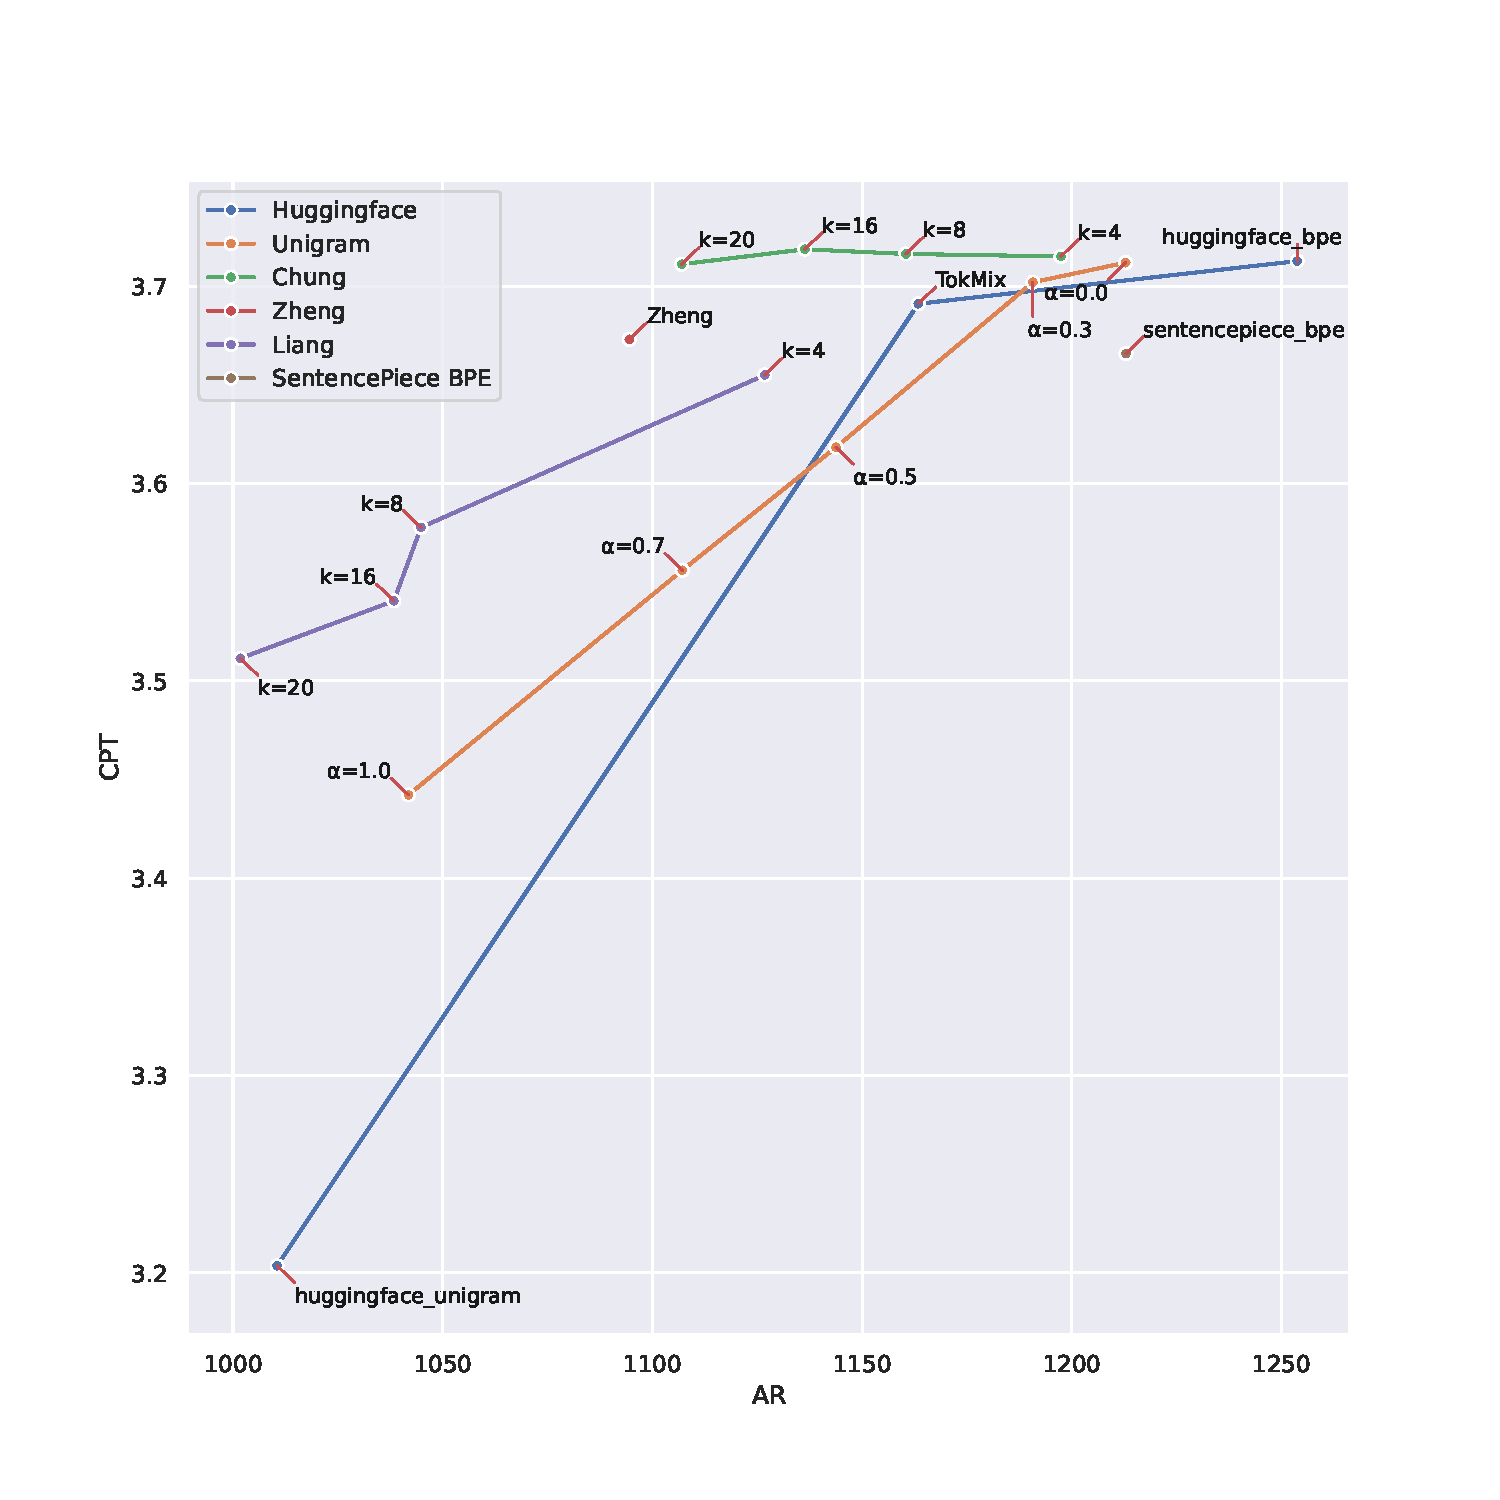
\includegraphics[width=\textwidth]{figures/all_tokenizers_AR_vs_CPT.pdf}
    \caption{all tokenizers AR vs CPT}
    \label{fig:all_tokenizers_AR_vs_CPT}
\end{figure}

\begin{figure}[H]
    \centering
    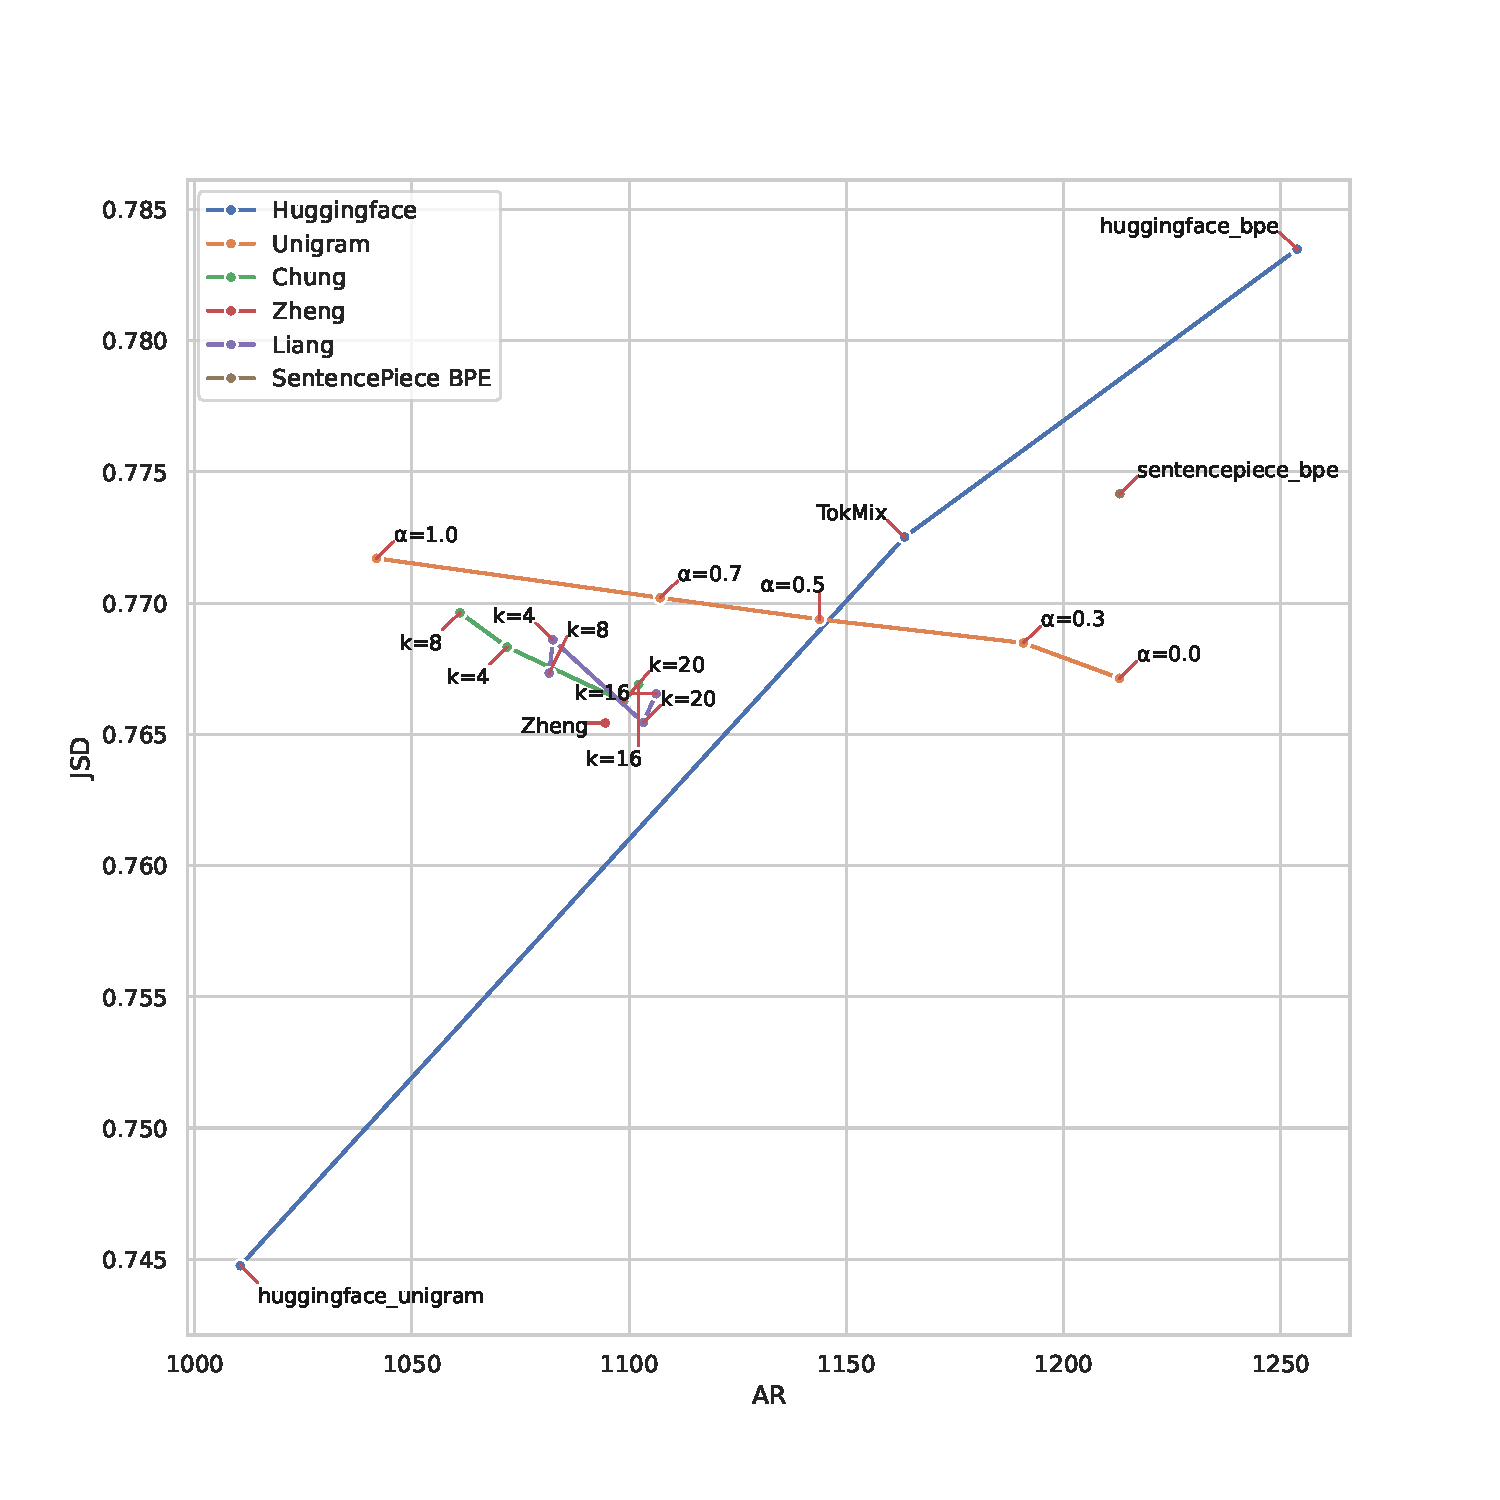
\includegraphics[width=\textwidth]{figures/all_tokenizers_AR_vs_JSD.pdf}
    \caption{all tokenizers AR vs JSD}
    \label{fig:all_tokenizers_AR_vs_JSD}
\end{figure}

\begin{figure}[H]
    \centering
    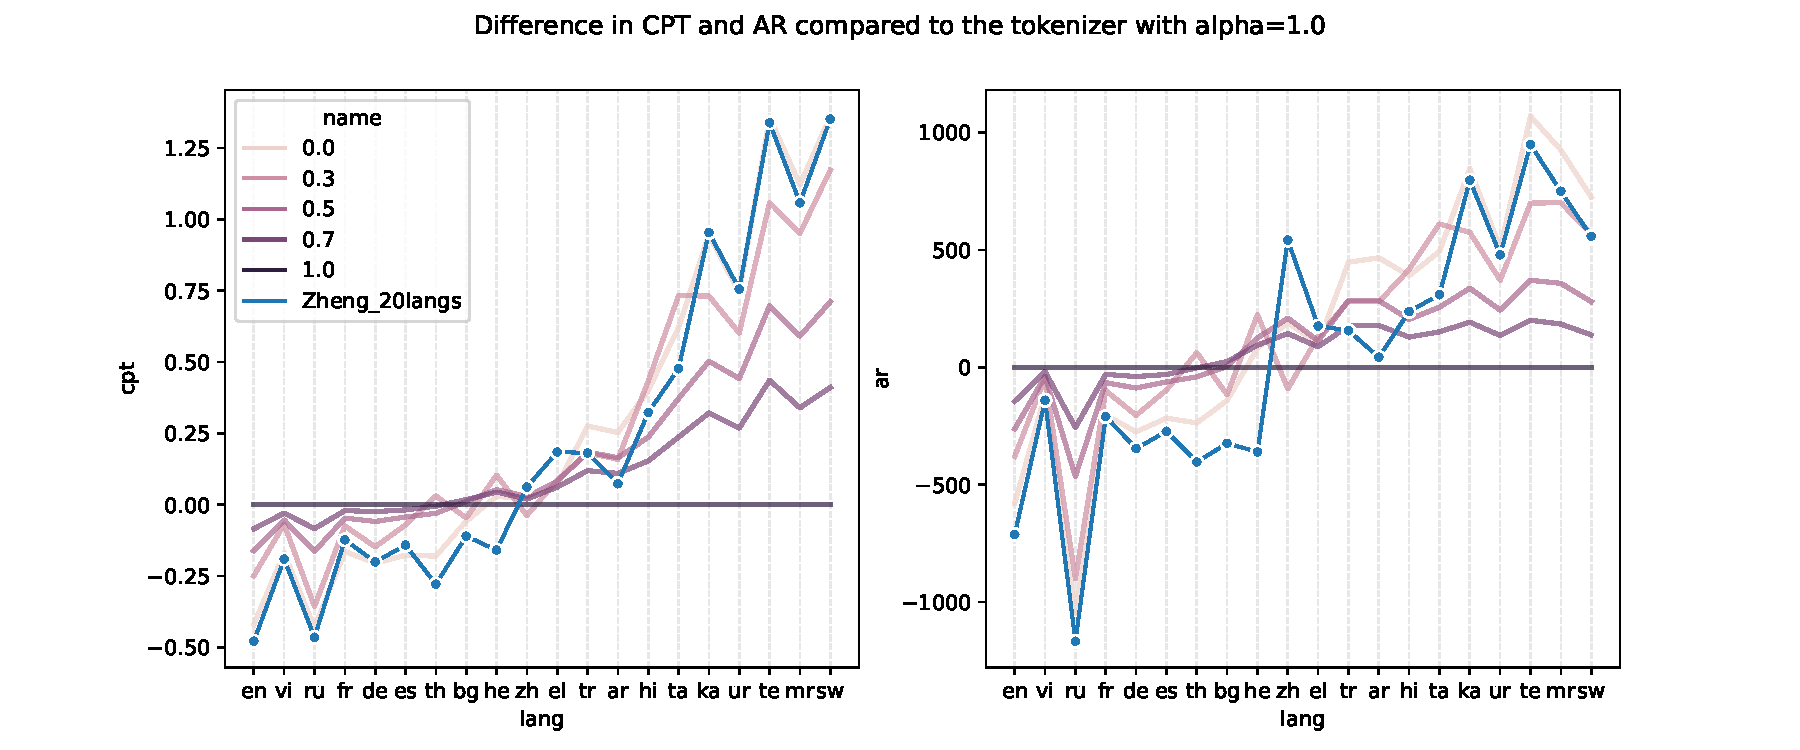
\includegraphics[width=\textwidth]{figures/zheng_vs_alphas.pdf}
    \caption{fefefef.}
    \label{fig:zheng_vs_alphas}
\end{figure}

\begin{figure}[H]
    \centering
    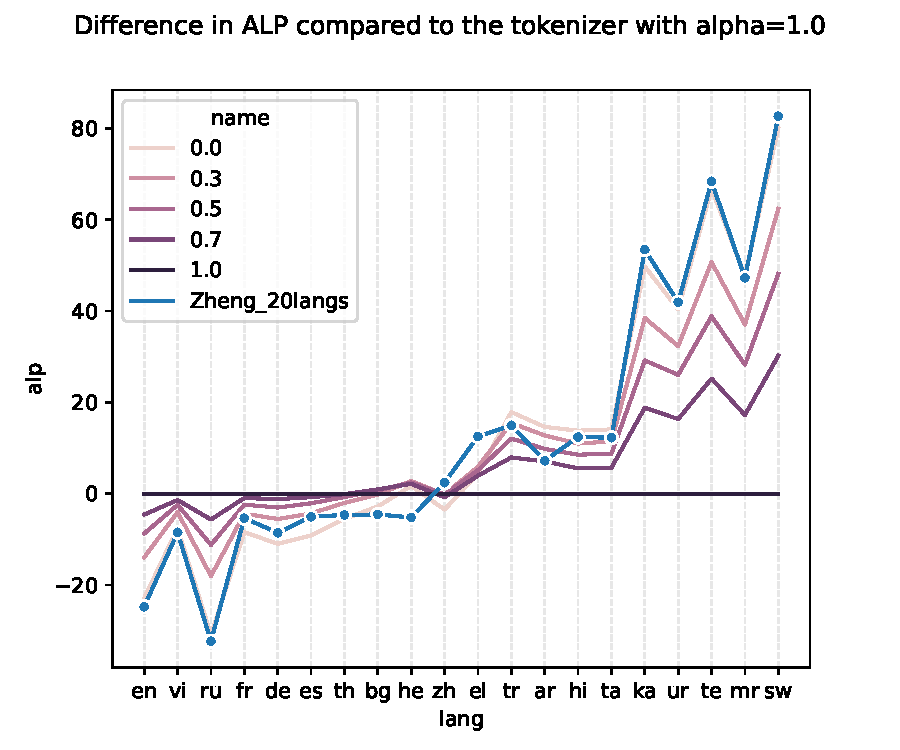
\includegraphics[width=\textwidth]{figures/zheng_vs_alphas_alp.pdf}
    \caption{fefefef.}
    \label{fig:zheng_vs_alphas_alp}
\end{figure}


\begin{figure}[H]
    \centering
    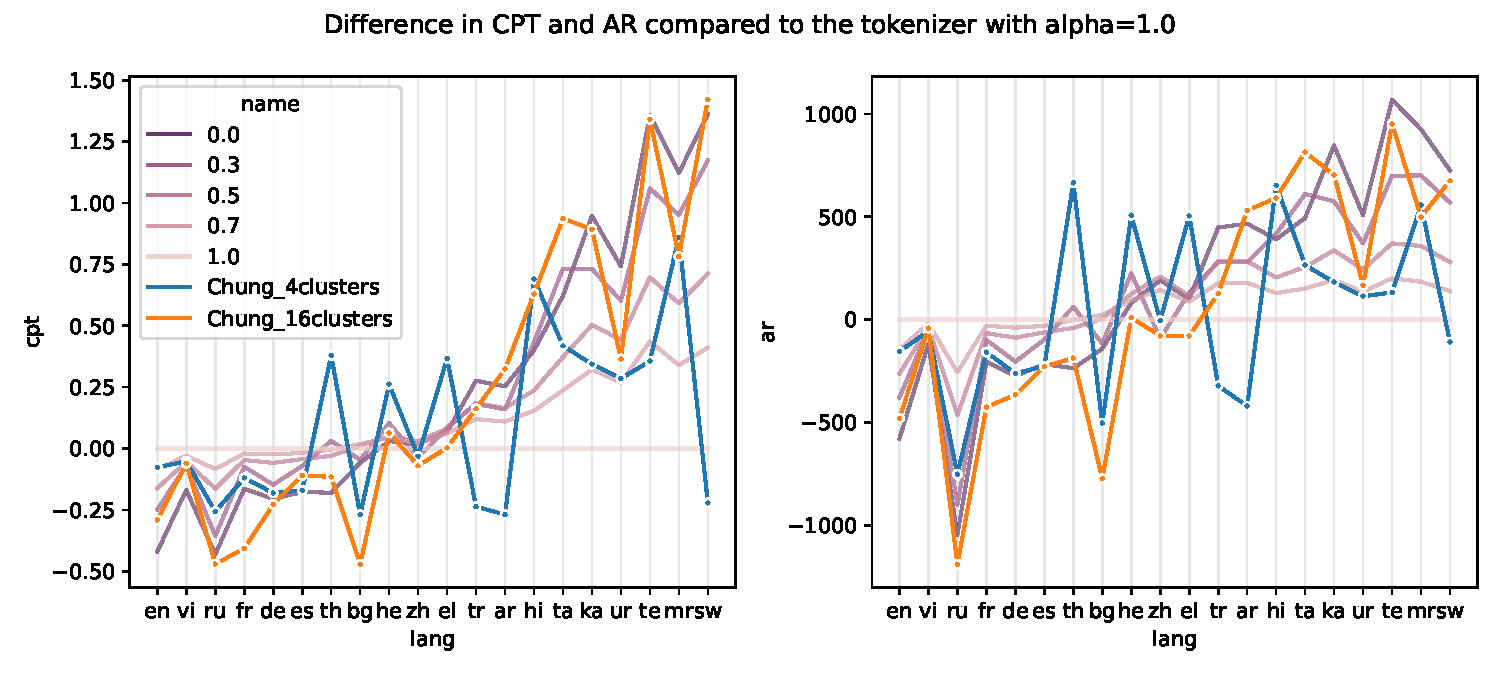
\includegraphics[width=\textwidth]{figures/chung_vs_alphas.pdf}
    \caption{fefefef.}
    \label{fig:chung_vs_alphas}
\end{figure}

\begin{figure}[H]
    \centering
    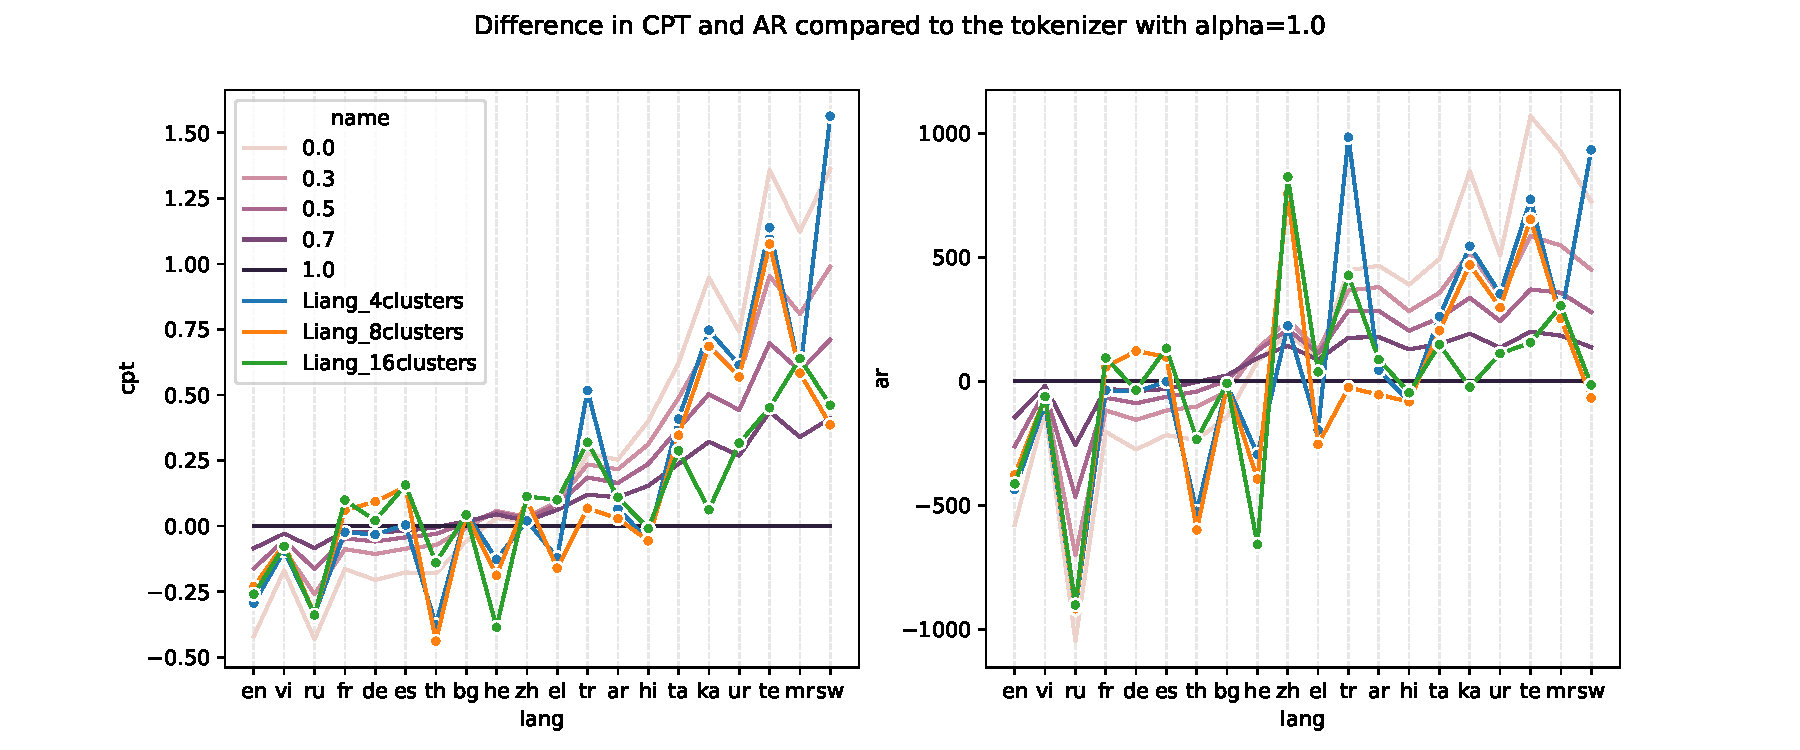
\includegraphics[width=\textwidth]{figures/liang_vs_alphas.pdf}
    \caption{fefefef.}
    \label{fig:liang_vs_alphas}
\end{figure}

\subsection{Balancing methods and vocabulary overlap}
\section{Comparison of balancing methods on downstream tasks}


\begin{figure}[H]
    \centering
    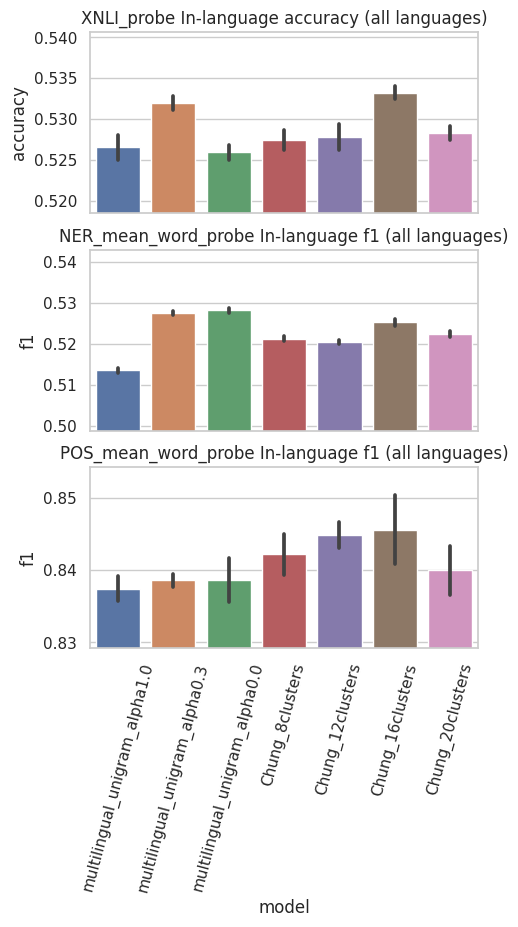
\includegraphics[width=\textwidth]{img/temp/probe_overall_inlanguage.png}
    \caption{probe overall inlanguage}
    \label{fig:probe_overall_inlanguage}
\end{figure}


\begin{figure}[H]
    \centering
    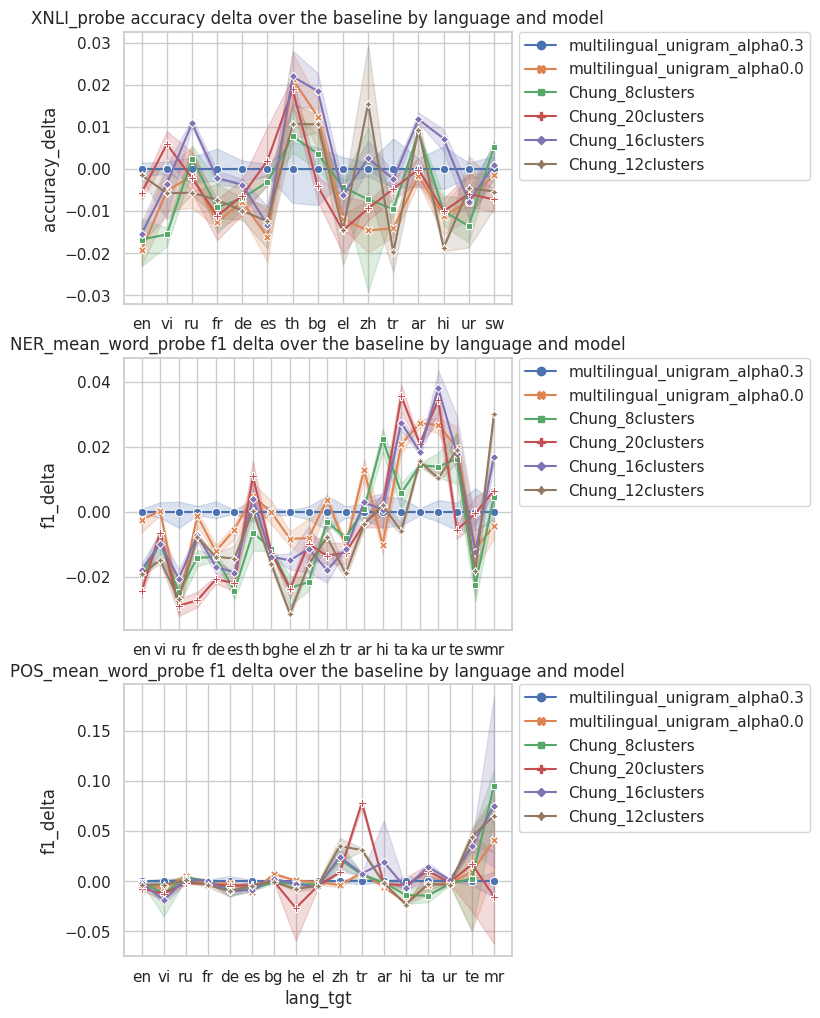
\includegraphics[width=\textwidth]{img/temp/probe_overall_inlanguage_over_baseline.png}
    \caption{probe overall inlanguage over baseline}
    \label{fig:probe_overall_inlanguage_over_baseline}
\end{figure}


\begin{figure}[H]
    \centering
    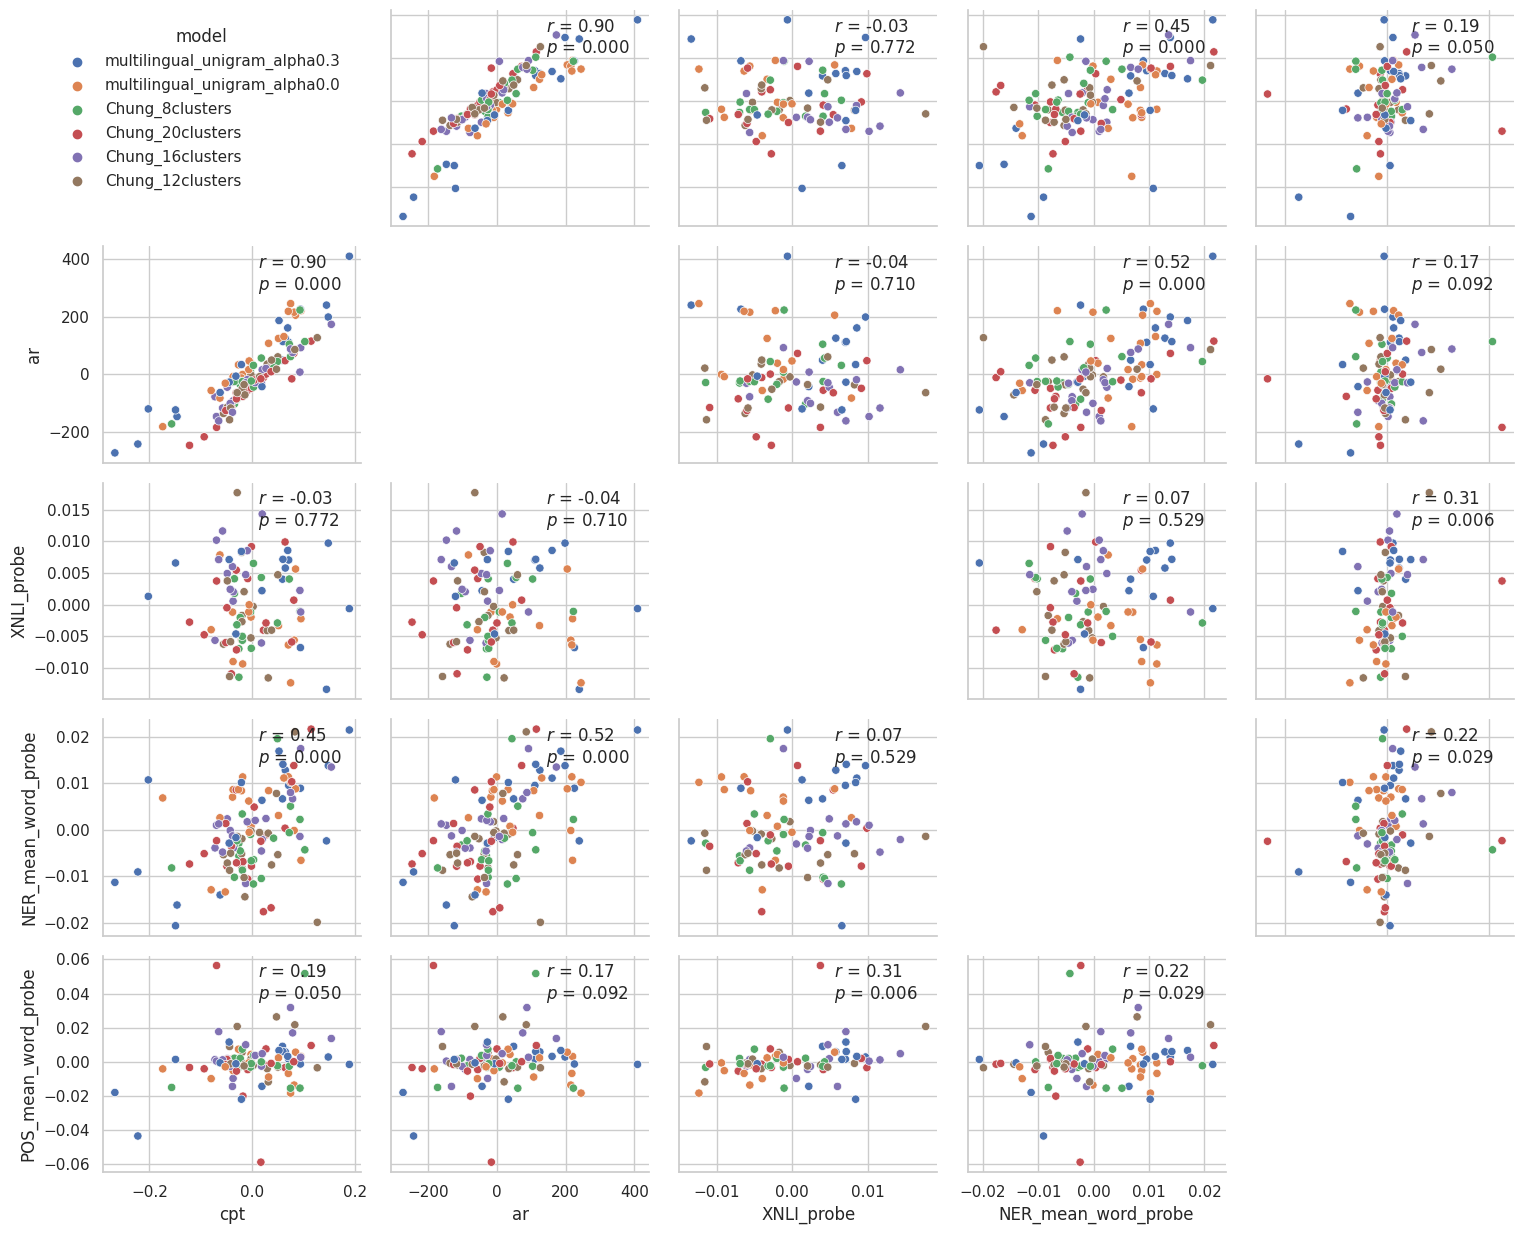
\includegraphics[width=\textwidth]{img/temp/probe_overall_inlanguage_scattermatrix.png}
    \caption{probe overall inlanguage scattermatrix}
    \label{fig:probe_overall_inlanguage_scattermatrix}
\end{figure}


\begin{figure}[H]
    \centering
    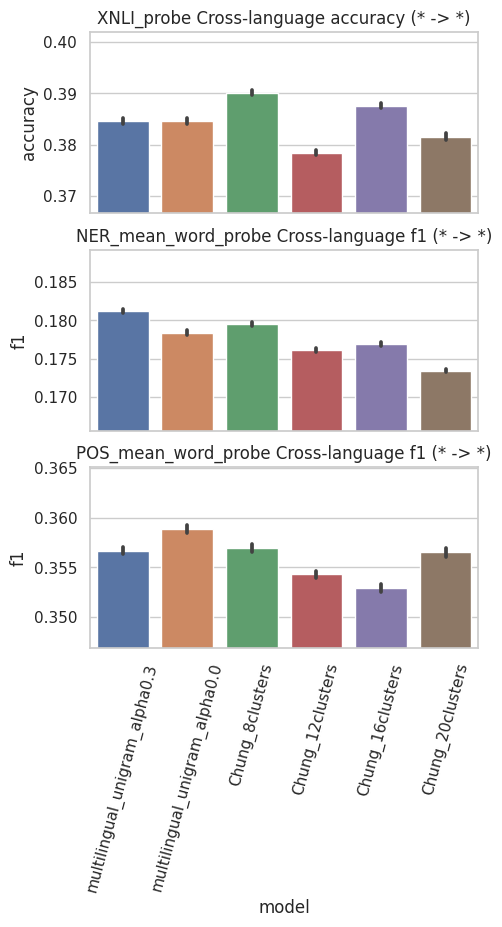
\includegraphics[width=\textwidth]{img/temp/probe_overall_crosslanguage.png}
    \caption{probe overall crosslanguage}
    \label{fig:probe_overall_crosslanguage}
\end{figure}


\begin{figure}[H]
    \centering
    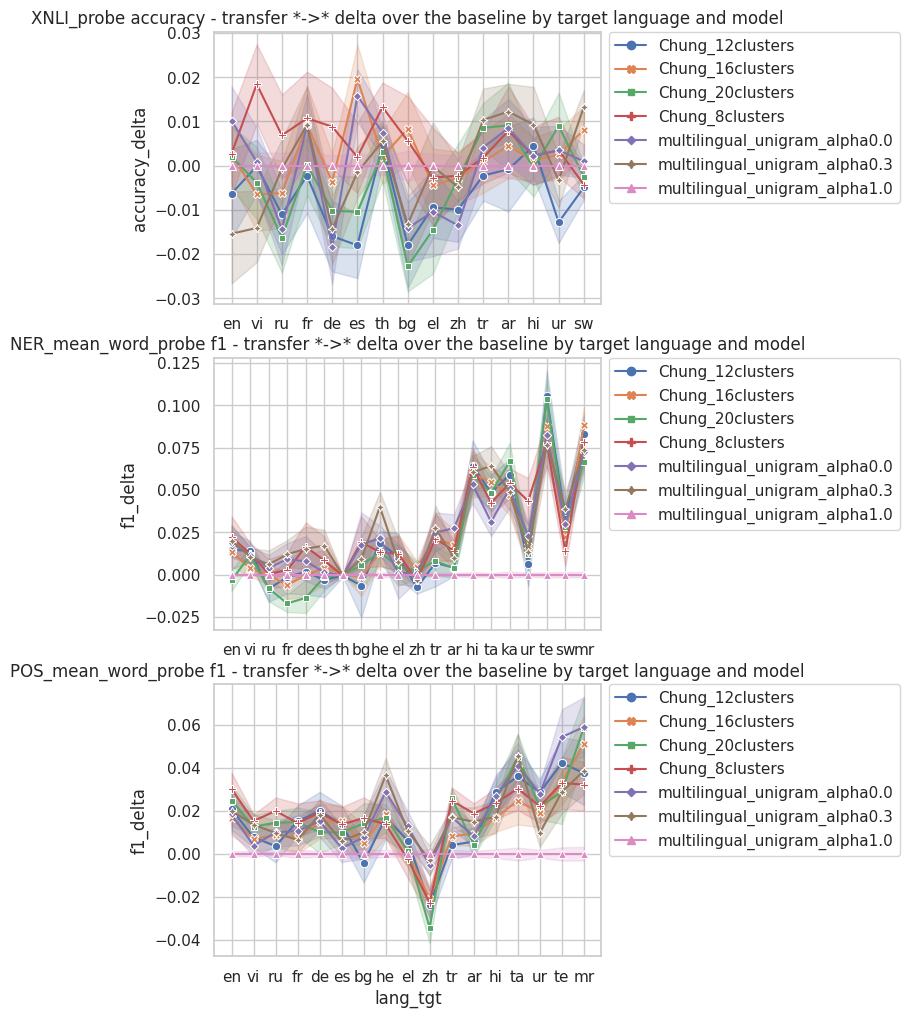
\includegraphics[width=\textwidth]{img/temp/probe_overall_crosslanguage_over_baseline.png}
    \caption{probe overall crosslanguage over baseline}
    \label{fig:probe_overall_crosslanguage_over_baseline}
\end{figure}


\begin{figure}[H]
    \centering
    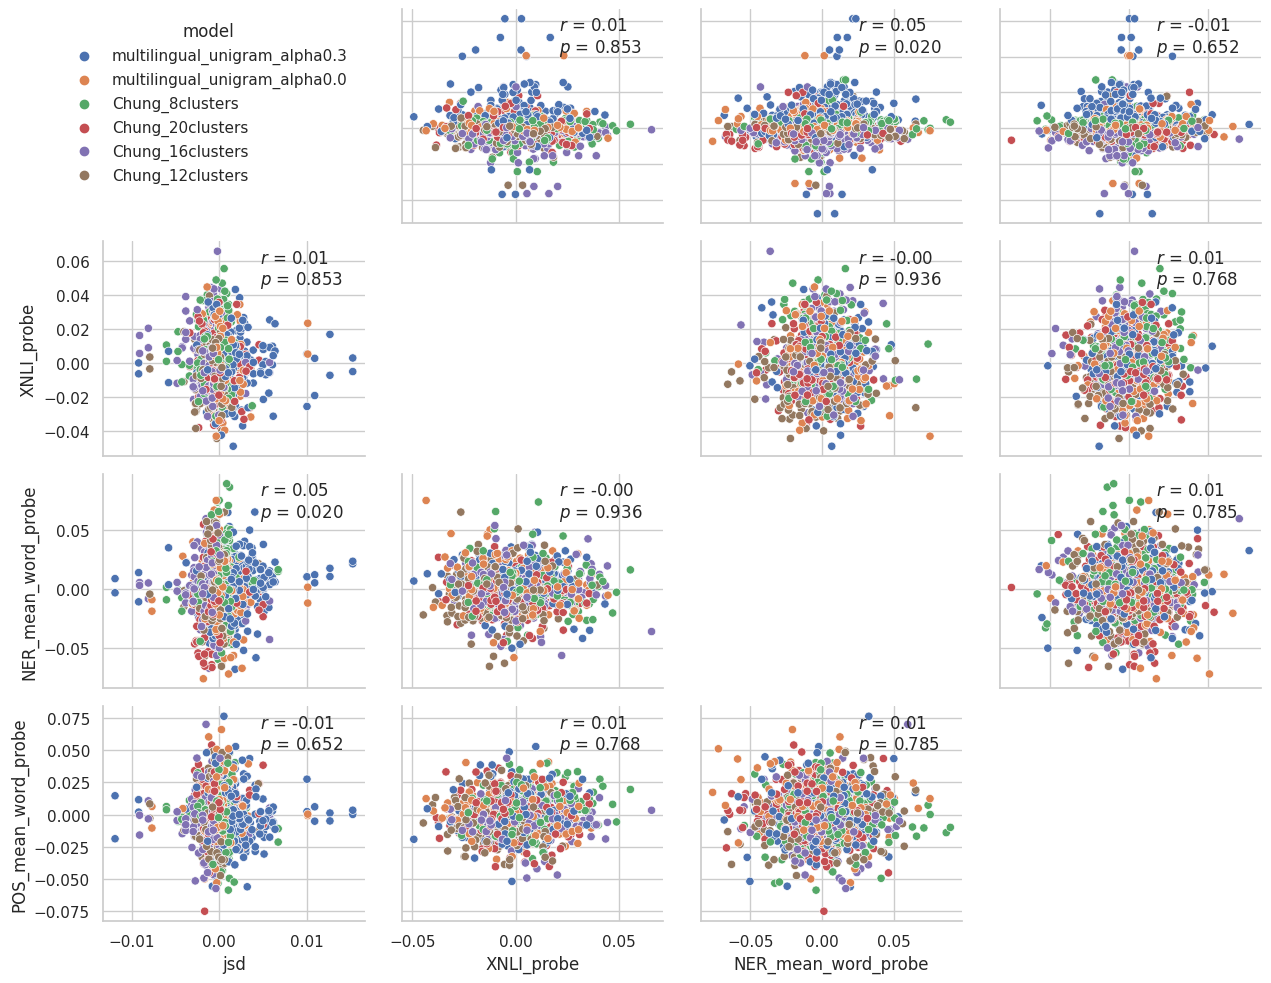
\includegraphics[width=\textwidth]{img/temp/probe_overall_crosslanguage_scattermatrix.png}
    \caption{probe overall crosslanguage scattermatrix}
    \label{fig:probe_overall_crosslanguage_scattermatrix}
\end{figure}

% visualization idea:

% - visualization of tokenizer balance difference is too noisy to see the differences between methods
%     - smoothing num_lines_per_language vs cpt
%     - or fitting a line
%     - something that highlights if one balancing method is better than another

% \section{Preliminary experiments}
% \subsection{The importance of training data size}
% \subsection{Differences in tokenizer implementations}
% \section{Reproduction of baselines}
% \section{Document-level clustering method}
% \section{Extrinsic evaluation}


% - replication of the previous work
%     - Chung
%         - reproductions in Overlap-based Vocabulary Generation Improves Cross-lingual Transfer Among Related Languages

%     - Liang
%         - they use 900k vocab, they compare their model to XLM-R which is not fair!
%             - they discuss it in section 6.4
%         - reproductions: https://github.com/stefan-it/xlm-v-experiments
%             - For XQuAD they did not reproduce the improvements
%             - For MasakhaNER they reproduced the improvements
%             - TODO: could use bootstrapping to show whether the improvements are significant

% replications of Chung, Liang
% https://github.com/stefan-it/xlm-v-experiments

% - our beta experiments point to the randomness of the output - the smooth sweep across the beta values seems to produce quite noisy outpus
